\documentclass[conference]{IEEEtran}
\IEEEoverridecommandlockouts
% The preceding line is only needed to identify funding in the first footnote. If that is unneeded, please comment it out.
\usepackage{cite}

\usepackage[utf8]{inputenc}
\usepackage{subcaption}
\usepackage{dcolumn}
\usepackage{placeins}
\usepackage{hyperref}
\usepackage{pdfpages}
\hypersetup{
    colorlinks=true,
    linkcolor=blue,
    filecolor=magenta,      
    urlcolor=cyan,
}
 
\urlstyle{same}

\title{A Network Intrusion Detection System realized using Neural Networks}
\author{Alvise de' Faveri Tron\\
\textit{Advanced Data Exploration and Optimization}\\
\textit{EISTI}}
\date{December 2019}

\usepackage{natbib}
\usepackage{graphicx}

\usepackage{amsmath,amssymb,amsfonts}
\usepackage{algorithmic}
\usepackage{graphicx}
\usepackage{textcomp}
\usepackage{xcolor}
\def\BibTeX{{\rm B\kern-.05em{\sc i\kern-.025em b}\kern-.08em
    T\kern-.1667em\lower.7ex\hbox{E}\kern-.125emX}}
\begin{document}

\title{A Network Intrusion Detection System realized using Neural Networks\\
}

\author{\IEEEauthorblockN{1\textsuperscript{st} Alvise de' Faveri Tron}
\IEEEauthorblockA{\textit{Advanced Data Exploration and Optimization} \\
\textit{EISTI}\\
Cergy, France \\
defaveritr@eisti.eu}
}

\maketitle

\begin{abstract}

Faced with the increase of more advanced attacks targeting information systems, a defense system has become vital. An intrusion detection system provides a first line of defense. 
A intrusion detection system monitor events within an information system or in one of the organs of the information system
The objective of this research project is to design a lightweight intrusion detection system using artificial intelligence techniques, in particular deep learning techniques. 
The neural network will be trained and tested with the NSL KDD dataset.
\end{abstract}

\begin{IEEEkeywords}
Neural Networks, Intrusion Detection, Computer Security
\end{IEEEkeywords}

%-------
\section{Introduction}
\label{chapter:introduction}
%-------
\subsection{Intrusion Detection Systems}

Intrusion Detection is a key concept in modern computer networks security. Rather than protecting a network against known malware by preventing the connection to enter the network, as in Intrusion Prevention Systems, Intrusion Detection is aimed to analyzing the current state of a network in real-time and identify potential anomalies that are happening in the system, reporting them as soon as they are identified. This enables the possibility to detect previously unknown malware \cite{ids}.

Intrusion Detection Systems are generally classified according to the following categories \cite{idsclass}:

\begin{itemize}
    \item \textbf{Anomaly Detection vs Misuse Detection}:  In misuse detection, each instance in a data set is labeled as ‘normal’ or ‘intrusive’ and a learning algorithm is trained over the labeled data. Anomaly detection approaches, on the other hand, build models of normal data and detect deviations from the normal model in observed data.
    \item  \textbf{Network-based vs Host-based}: Network intrusion detection systems (NIDS) are placed at a strategic point or points within the network to monitor traffic to and from all devices on the network, while Host intrusion detection systems (HIDS) run on individual hosts or devices on the network.
\end{itemize}

The object of this work, in particular, is the production of a NIDS trained on labelled data which is able to recognize suspect behaviour in a network and classify each connection as normal or anomalous.

%-------
\subsection{Artificial Neural Networks}

Artificial Neural Networks are supervised machine learning algorithms inspired by the human brain. The main idea is to have many simple units, called \textit{neurons}, organized in \textit{layers}. In particular, in a feed-forward artificial neural network all neurons of a layer are connected to all the neurons of the following layer, and so on until the last layer, which contains the \textit{output} of the neural network.

This kind of networks are a popular choice among Data Mining techniques in now days, and have already been proven to be a valuable choice for Intrusion Detection \cite{nnids,nnids2}.

In this work we are using feed-forward neural networks trained on the NSL-KDD dataset to classify network connections as belonging to one of two possible categories: \textit{normal} or \textit{anomalous}. The goal of this work is to maximize the accuracy in recognizing new data samples, while also avoid \textit{overfitting}, which happens when the algorithm is too attached to the data it learned and is not capable of correctly generalizing on previously unseen data.

%-------
\subsection{The NSL-KDD Dataset}

The dataset used for training and validation of the neural network is the NSL-KDD dataset, which is an improved version of the KDD CUP '99 dataset \cite{nslkdd, nslkdd2}. This data set is a well known benchmark in the field of Network Intrusion Detection techniques, providing 42 features for each example and many anomalous examples.

The dataset has been taken from the University of New Brunswick's website.\cite{dataset}.

A detailed analysis of the dataset is provided in the next Section.

%-------
\section{Dataset Analysis}
\label{chapter:dataset}
This section provides a complete analysis of the NSL-KDD dataset.

%-------
\subsection{Dataset Summary}

The NSL-KDD dataset is provided in two forms: \texttt{.arff} files, with binary labels, and \texttt{.csv} files, with categorical labels for each instance.

Since the object of this work is to build a binary classifier, we will focus only on the \texttt{.arff} files. The provided \texttt{.arff} files are:

\begin{itemize}
    \item \textbf{KDDTrain+.ARFF}: The full NSL-KDD train set with binary labels in ARFF format
    \item \textbf{KDDTrain+\_20Percent.ARFF}: A 20\% subset of the KDDTrain+.arff file
    \item \textbf{KDDTest+.ARFF}: The full NSL-KDD test set with binary labels in ARFF format
    \item \textbf{KDDTest-21.ARFF}: A subset of the KDDTest+.arff file which does not include records with difficulty level of 21 out of 21
\end{itemize}

To avoid redundancy, we use only the \texttt{KDDTrain+.ARFF} and \texttt{KDDTest+.ARFF} files, which contain a total of about 148,500 entries.

Table~\ref{tab:summ} contains a summary of the most important attributes of the dataset.

\FloatBarrier

\begin{table}[!htb]
    \centering
    
    \begin{tabular}{|l|l|}
    \hline
    \multicolumn{2}{|c|}{\textbf{Summary}} \\ \hline
    train rows              & 125973             \\ \hline
    test rows               & 22544              \\ \hline
    total rows              & 148517             \\ \hline
    columns                 & 42                 \\ \hline
    duplicates              & 629                \\ \hline
    null values             & None               \\ \hline
    \end{tabular}
    \caption{Dataset Attributes}
    \label{tab:summ}
\end{table}
\FloatBarrier

%-------
\subsection{Features}
            
As for the features of this dataset, they can be broken down into 4 types (excluding the target column):

\begin{itemize}
    \item 4 Multi-Class
    \item 6 Binary
    \item 16 Discrete
    \item 15 Continuous
\end{itemize}

Tables~\ref{tab:cat} and \ref{tab:bin} contain a description of the categorical features of the dataset, while Tables~\ref{tab:disc} and \ref{tab:cont} describe the numerical features. Note that this definition slightly differs from the one provided by \cite{nslkdd}, since here categorical and binary features are listed regardless of their format (text or numeric). 
\begin{table}[]
    \centering
    \begin{tabular}{|l|l|}
    \hline
    \multicolumn{2}{|c|}{\textbf{Multi-Class Features}} \\ \hline
    \textit{Feature}     & \textit{Distinct Values} \\ \hline
    protocol\_type        & 3                \\ \hline
    service               & 70               \\ \hline
    flag                  & 11               \\ \hline
    su\_attempted	      & 3                \\ \hline
    \end{tabular}
    \caption{Multi-Class Features in the NSL-KDD dataset}
    \label{tab:cat}
\end{table}

\begin{table}[]
    \centering
    \begin{tabular}{|l|l|}
    \hline
    \multicolumn{2}{|c|}{\textbf{Binary Features}} \\ \hline
    \textit{Feature}     & \textit{Number of '0's} \\ \hline
    land	 & 99.98\%	 \\ \hline
    logged\_in	 & 59.72\%	 \\ \hline
    root\_shell	 & 99.85\%	 \\ \hline
    num\_outbound\_cmds	 & 100.00\%	 \\ \hline
    is\_host\_login	 & 99.99\%	 \\ \hline
    is\_guest\_login	 & 98.77\%	 \\ \hline
    \end{tabular}
    \caption{Binary Features in the NSL-KDD dataset}
    \label{tab:bin}
\end{table}

\begin{table}[]
    \centering
     \begin{tabular}{|l|l|l|}
    \hline
    \multicolumn{3}{|c|}{\textbf{Discrete Features}} \\ \hline
    \textit{Feature}     & \textit{Mean} & \textit{Stddev} \\ \hline
    wrong\_fragment   & 0.02      & 0.24  \\ \hline
    urgent   & 0.00      & 0.02  \\ \hline
    count    & 83.34     & 116.76    \\ \hline
    srv\_count    & 28.25     & 75.37     \\ \hline
    dst\_host\_count   & 183.93    & 98.53     \\ \hline
    dst\_host\_srv\_count   & 119.46    & 111.23    \\ \hline
    duration     & 276.78    & 2.46k   \\ \hline
    src\_bytes    & 40.22k      & 5.4M    \\ \hline
    dst\_bytes    & 17.08k     & 3.7M    \\ \hline
    hot  & 0.19      & 2.01  \\ \hline
    num\_failed\_logins    & 0.00      & 0.07  \\ \hline
    num\_compromised  & 0.26      & 22.23     \\ \hline
    num\_root     & 0.27      & 22.69     \\ \hline
    num\_file\_creations   & 0.01      & 0.52  \\ \hline
    num\_shells   & 0.00      & 0.03  \\ \hline
    num\_access\_files     & 0.00      & 0.10  \\ \hline
    \end{tabular}
    \caption{Discrete Features in the NSL-KDD dataset}
    \label{tab:disc}
\end{table}

\begin{table}[]
    \centering
    \begin{tabular}{|l|l|l|}
    \hline
    \multicolumn{3}{|c|}{\textbf{Continuous Features}} \\ \hline
    \textit{Feature}     & \textit{Mean} & \textit{Stddev} \\ \hline
    serror\_rate  & 0.26      & 0.43  \\ \hline
    srv\_serror\_rate  & 0.26      & 0.43  \\ \hline
    rerror\_rate  & 0.14      & 0.34  \\ \hline
    srv\_rerror\_rate  & 0.14      & 0.34  \\ \hline
    same\_srv\_rate    & 0.67      & 0.44  \\ \hline
    diff\_srv\_rate    & 0.07      & 0.19  \\ \hline
    srv\_diff\_host\_rate   & 0.10      & 0.26  \\ \hline
    dst\_host\_same\_srv\_rate   & 0.53      & 0.45  \\ \hline
    dst\_host\_diff\_srv\_rate   & 0.08      & 0.19  \\ \hline
    dst\_host\_same\_src\_port\_rate  & 0.15      & 0.31  \\ \hline
    dst\_host\_srv\_diff\_host\_rate  & 0.03      & 0.11  \\ \hline
    dst\_host\_serror\_rate     & 0.26      & 0.43  \\ \hline
    dst\_host\_srv\_serror\_rate     & 0.25      & 0.43  \\ \hline
    dst\_host\_rerror\_rate     & 0.14      & 0.32  \\ \hline
    dst\_host\_srv\_rerror\_rate     & 0.14      & 0.34  \\ \hline
    \end{tabular}
    \caption{Continuous Features in the NSL-KDD dataset}
    \label{tab:cont}
\end{table}



%-------
\subsection{Categories Distributions}

The NSL-KDD dataset contains a few binary and multi-class categorical features, which are used to label each connection with its protocol, service and other useful characteristics, e.g. if the user tried to gain super-user access or if he spawned a root shell during its connection. 

The figures contained in the next page describe, for each categorical feature, how many occurrences of each label are present in both the train and the test set. Note that \textit{class}, \textit{protocol\_type}, \textit{service} and \textit{flag} features contain textual values, while all other categories are expressed by a number.

As we can see, the target variable (\textit{class}) has a nearly even distribution of its values (\textit{normal} and \textit{anomalous)} throughout the dataset, meaning that there are a lot of anomalous examples that can be used for training. As opposed to this, we can see that some of the categories are not evenly distributed, having more than 99\% of the samples belonging to just one class. This kind of analysis can be useful during the feature selection step.


\FloatBarrier

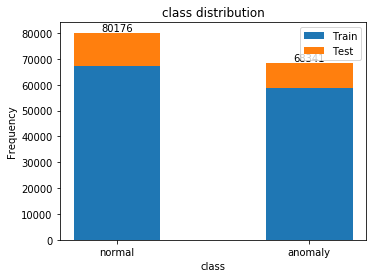
\includegraphics[width=0.9\linewidth]{img/cat6.png}


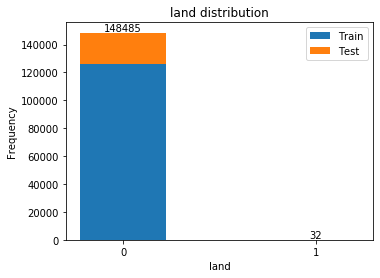
\includegraphics[width=0.9\linewidth]{img/cat1.png}

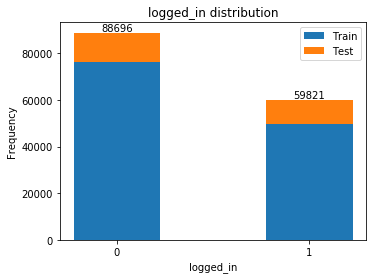
\includegraphics[width=0.9\linewidth]{img/cat2.png}

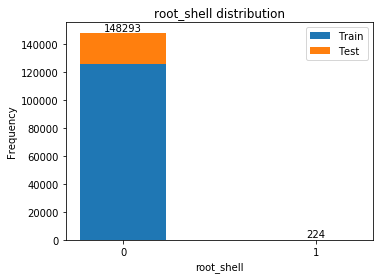
\includegraphics[width=0.9\linewidth]{img/cat3.png}

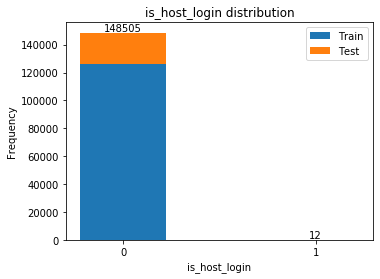
\includegraphics[width=0.9\linewidth]{img/cat4.png}

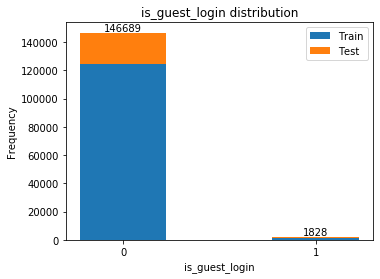
\includegraphics[width=0.9\linewidth]{img/cat5.png}

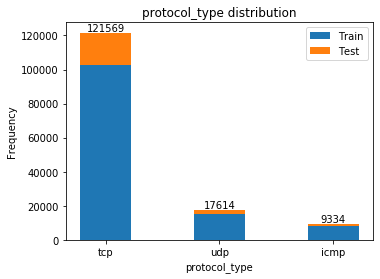
\includegraphics[width=0.9\linewidth]{img/cat7.png}
      
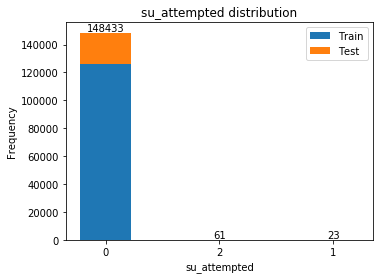
\includegraphics[width=0.9\linewidth]{img/cat8.png}

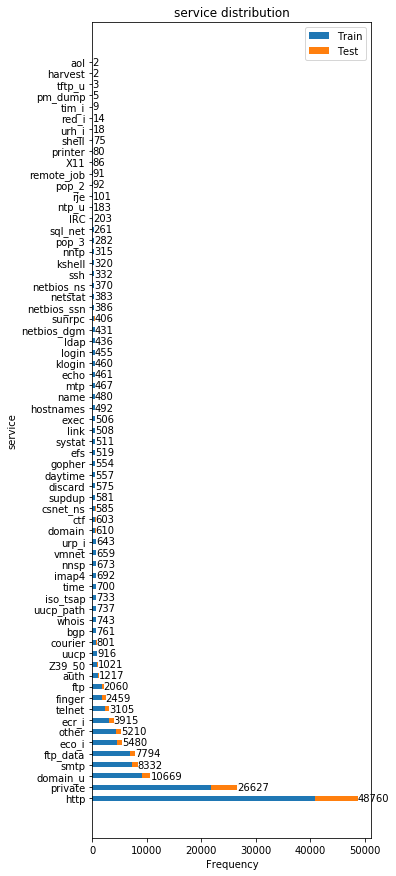
\includegraphics[width=0.9\linewidth]{img/cat10.png}

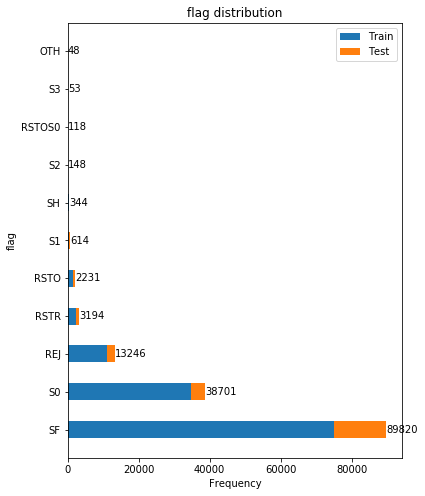
\includegraphics[width=0.9\linewidth]{img/cat9.png}

\FloatBarrier

%-------
\subsection{Numerical Data Distribution}

Numerical features have very different meanings in this dataset, and consequently different ranges. Continuous features are used for rates (e.g. error rates) and discrete features give information about the number of bytes in the packet, the connection duration, the number of reconnections and many other variables.

Figure~\ref{fig:contdist} represents the normalized dataset: each column's value has been normalized between 0 and 1 in order to visualize how the different values of each feature are distributed. Note that this normalization takes into account both the train and the test set, hence it can be used only for data analysis. Section~\ref{subsec:norm} describes how the train and test set have been normalized for learning. 

\begin{figure}[h]
    \centering
    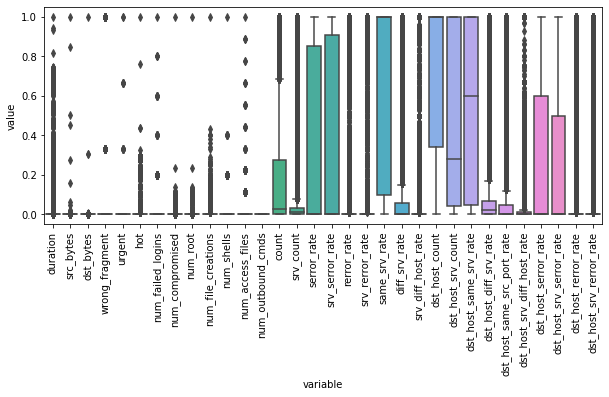
\includegraphics[width=\linewidth]{img/box-norm.png}
    \caption{Distribution of discrete and continuous values in the normalized dataset.}
    \label{fig:contdist}
\end{figure}
\FloatBarrier


%-------
\subsection{Correlation Matrix}

As a final step of the data analysis, we ran a correlation analysis for all the features of the dataset. Figure~\ref{fig:corr} illustrates the correlation matrix. Focusing on the \textit{class} column, we can see how each feature is correlated with the target variable, either directly or inversely. This analysis can be extremely useful when performing feature selection to estimate how many important features there are in the dataset.

\FloatBarrier

\begin{figure}[h]
    \centering
    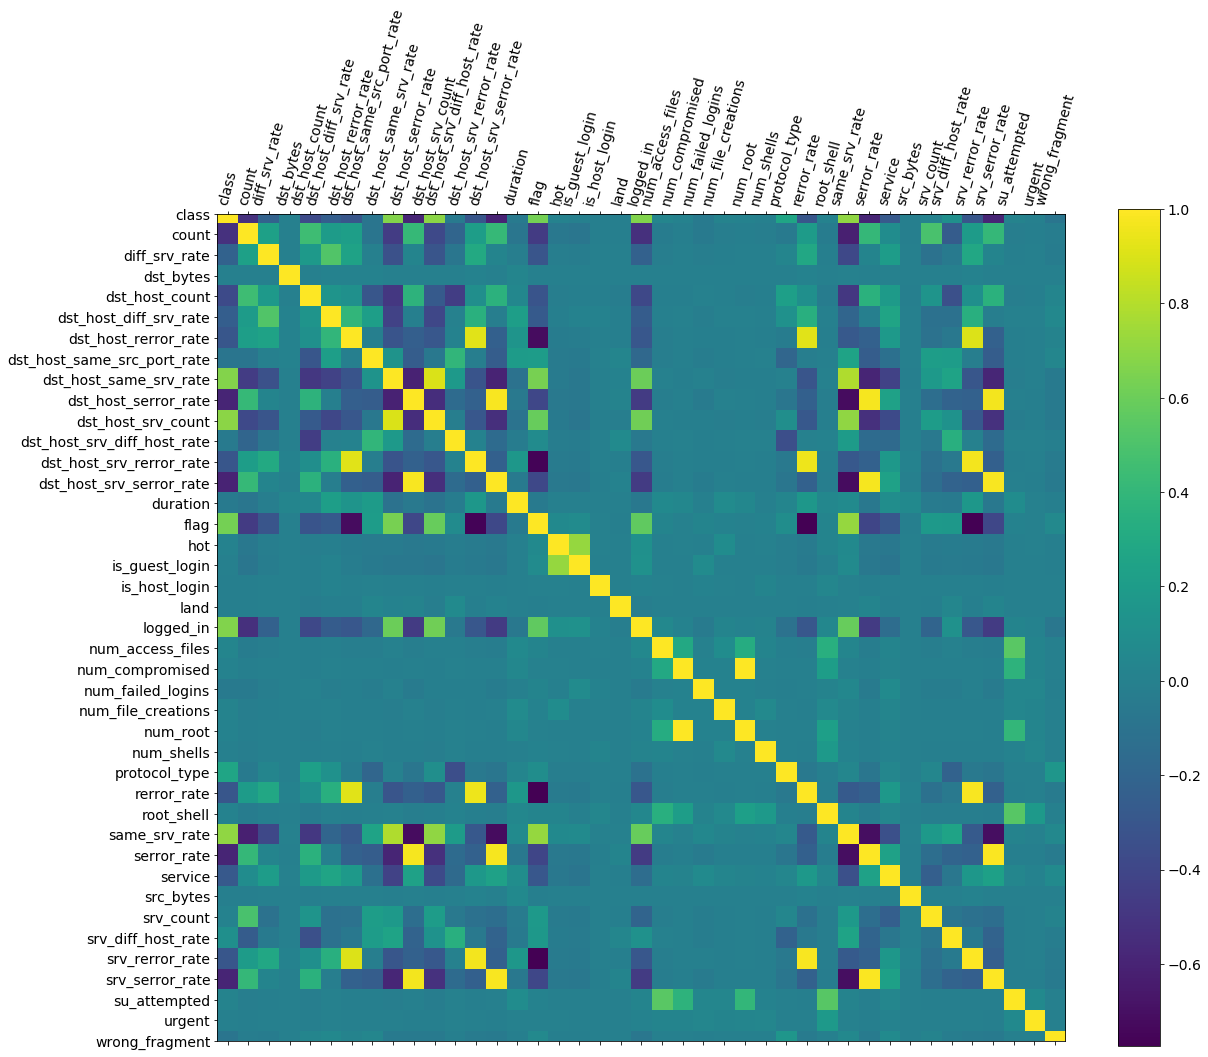
\includegraphics[width=0.9\linewidth]{img/corr1.png}
    \caption{Correlation matrix between each feature of the dataset. A brighter color means higher correlation.}
    \label{fig:corr}
\end{figure}

\FloatBarrier

%-------
\section{Data Preparation}
\label{chapter:dat-preparation}
In this Section we will describe all the techniques used for cleaning and preparing the data for the learning phase.

%-------
\subsection{Data Cleaning}

Since the NSL-KDD dataset is already an enhanced version of the older KDD '99 CUP dataset, little additional cleaning had to be performed: the set had already been cleaned from redundant data and null values \cite{nslkdd}. Also, the ratio between normal and anomalous entries is good for machine learning purposes.

The only step taken at this stage, a part from loading the \texttt{.arff} files and decoding strings using UTF-8, was to change all the entries with \textit{http\_XXX} as their  \texttt{service} values into \textit{http}, where \textit{XXX} denotes the port number.

This decision was taken since the port of an http connection, which is specified in the protocol string only for some entries, is very unlike to be correlated with an anomalous behaviour in a general case. Also, leaving this distinction could lead to new http connections on previously unseen ports to not be recognized correctly by the algorithm.

This cleaning has later been proven to be an effective solution for partially reducing overfitting.

%-------
\subsection{Categorical Columns Encoding}

After cleaning the dataset, the second step was to convert all categorical columns into one-hot encoded columns. This means that, for each distinct value of each categorical column, a new column is generated, contaning '1' for the rows belong to that category and '0' elsewhere.

This kind of encoding is the most popular choice when it comes to preparing data for ANN learning \cite{encoding}. This is done to prevent the algorithm from interpreting categories as numbers, which can lead to problems like the algorithm considering a category the mean of other two categories etc.

The affected columns in particular are:

\begin{itemize}
    \item service
    \item protocol\_type
    \item su\_attempted
    \item flag
    \item class (target variable)
\end{itemize}

The dataset resulting from this encoding contains \textbf{124} columns, of which 2 are the target columns.

Note that, a part from the target column, all other binary columns where not affected by the encoding. This is to avoid redundant columns, since binary features would have two corresponding encoded columns in which one can be directly inferred by observing the other.

%-------
\subsection{Normalization}
\label{subsec:norm}

Having encoded the categorical columns, now the numerical columns have to be treated. In particular, it was decided to apply MinMax \cite{minmax} normalization to both discrete and continuous columns. The normalization process has been accomplished as follows: 

\begin{itemize}
    \item Fit the model onto the train set
    \item Transform the train set
    \item Transform the test set (with the same normalization model)
\end{itemize}

Figure~\ref{fig:trainnorm} describes the distribution of the numerical values in the train set after normalization, while Figure~\ref{fig:testnorm} illustrates the same transformation applied to the test set. As we can see, all values in the train set are correctly normalized between 1 and 0, while the test set contains some values that are greater than the maximum found on the train set, hence their normalized values is greater than 1.


\begin{figure}[h]
    \centering
    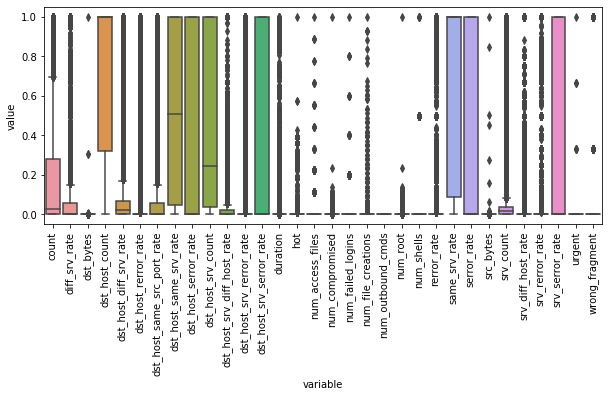
\includegraphics[width=\linewidth]{img/box_train.png}
    \caption{Distribution of numerical values in the normalized train set.}
    \label{fig:trainnorm}
\end{figure}


\begin{figure}[h]
    \centering
    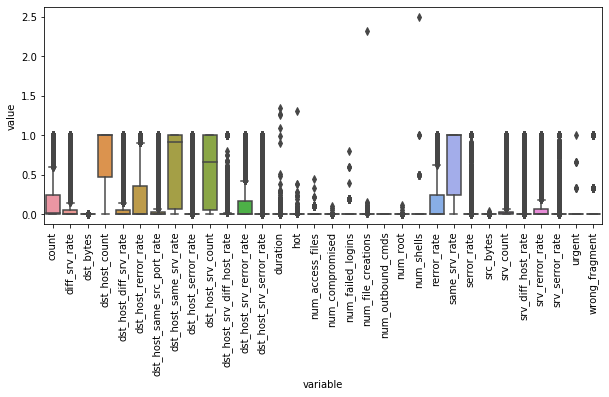
\includegraphics[width=\linewidth]{img/box_test.png}
    \caption{Distribution of numerical values in the normalized test set.}
    \label{fig:testnorm}
\end{figure}

\FloatBarrier

%-------
\section{Feature Selection}
\label{chapter:feature-selection}
Since the one-hot encoding increased considerably the number of features, some feature selection is needed to reduce the problem's complexity and reduce overfitting. If not correctly performed, feature selection can introduce some penalties in terms of the accuracy of the final output. A further discussion and comparision of the different models can be found in Section~\ref{chapter:validation}.

For this work, two different feature selection techniques have been chosen: ExtraTreeClassification and Univariate Selection.

%-------
\subsection{ExtraTree Classifier}

ExtraTreeClassifier is a classification algorithm provided by python's  \texttt{scikit-learn} library \cite{extratree}, which employs the random forest method to build a classifier and evaluate the feature importance.

Figure~\ref{fig:classtree} shows the ranking of the 15 best features obtained when running the classifier on the train set.

\begin{figure}[h]
    \centering
    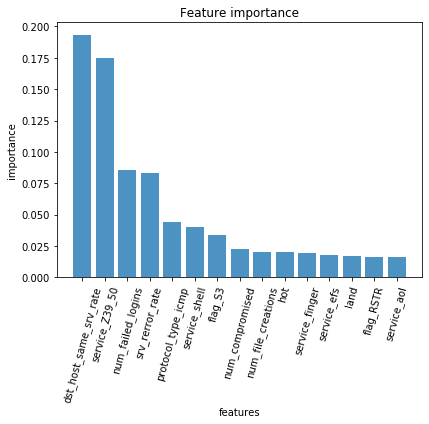
\includegraphics[width=0.7\linewidth]{img/extratree.png}
    \caption{Top 15 feature by importance as per ExtraTree Classifier ranking}
    \label{fig:classtree}
\end{figure}

%-------
\subsection{Univariate Selection}

Univariate feature selection is another method provided by the \texttt{scikit-learn} collection: it examines each feature individually to determine the strength of the relationship of the feature with the response variable \cite{univ}.

Figure~\ref{fig:classuniv} shows the best 15 features found with Univariate Selection. 

\begin{figure}[h]
    \centering
    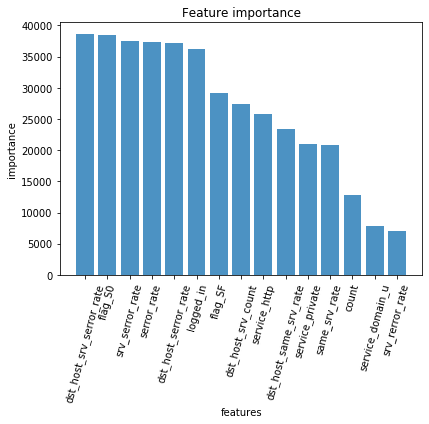
\includegraphics[width=0.7\linewidth]{img/univ.png}
    \caption{Top 15 feature by importance as per Univariate Selection ranking}
    \label{fig:classuniv}
\end{figure}

\FloatBarrier

%-------
\section{The Model}
\label{chapter:the-nn-model}
This Section describes how the Neural Network models where built and how the learning hyperparameters where set.

%-------
\subsection{Project Environment}

This project has been carried out using python3.6. To build the ANN model, the Keras library has been employed, with TensorFlow as a backend. The whole project has been developed on a Jupyter Notebooks project hosted on Google Colab \cite{project}. 

%-------
\subsection{Building the Neural Network}

The approach for constructing the neural network for this work has been to try different combinations of layers and see how each model performs in terms of accuracy and loss, comparing these two metrics for the train and test set.

All neural networks have been implemented in Keras \cite{kerass} using the Sequential (i.e. feed-forward) model and Dense (i.e. fully interconnected) layers. Following the work of \cite{deepshallow}, the tested models consists of both \textit{shallow} networks and \textit{deep} networks with 2 hidden layers.


%-------
\subsection{Hyperparameters}

The hyperparameters regarding the optimization and learning of each model have been mostly kept at the default values provided by Keras \cite{keras}. These are some of the defaults that Keras provides:

\begin{itemize}
    \item Learning Rate: 0.001
    \item Dropout: None
    \item Optimization Algorithm: Adam
\end{itemize}

%-------
\subsection{Epochs}

Each model was trained with a fixed number of epochs (\textbf{150}) and batch size = \textbf{10} for comparison purposes. In future developments, fixed epochs could be substituted by early stopping to speed up the learning phase.

%-------
\subsection{Activation Function}

Finally, the chosen activation function for all layers is the \textbf{sigmoid} function, which has proven to outperform other tested solutions, like using \textit{relu} for the input layer or \textit{tanh} for the hidden layers. 





%-------
\section{Validation}
\label{chapter:validation}

Many models have been tested in order to compare different solutions and find the best fit for this task. This section provides a comparison between the performance of each neural network model.

Each model comes with a description of its shape (i.e. number of layers, units per layer etc.), the training history (loss and accuracy in each epoch) and the final results on the test set (confusion matrix).

%-------
\subsection{Train-Test Splitting}
\label{subsec:traintest}

The NSL-KDD dataset is already divided into a train set containing 125973 instances ($\approx 85\%$) and test set containing 22544 instances ($\approx 15\%$). We also use 15\% of the train set as \textit{dev} set, to keep track of the accuracy and loss of each model during the training phase.

The initial batch of models have been tested on the provided test set, according to the initial division. Nevertheless, during the the development of this work it was been noted that reshuffling the train and test set significantly improves the ANN performance: these results are given in Section~\ref{subsec:porcata} .

The data normalization has not been performed on the entire dataset, but separately for the train and the test set using a normalization algorithm that was fitted on the train set. This ensures that the training of the model is not affected by the values that are in the test set.

%-------
\subsection{Evaluation Metrics}
\label{subsec:traintest}

The most common evaluation metrics for IDS, as reported by \cite{nslkdd2}, are \textit{Attack Detection Rate (DR)} and \textit{False Alarm Rate (FAR)}.

$$DR = \frac{TP}{TP+FN}$$

$$FAR = \frac{FP}{FP+TN}$$

We can calculate these metrics from the confusion matrix, which is represented by the following terms.

\begin{itemize}
    \item True Positive (TP): the instance is correctly predicted as an attack.
    \item True Negative (TN): correctly predicted as a non-attack or normal instance.
    \item False Positive (FP): a normal instance is wrongly predicted as attacks. 
    \item False Negative (FN): an actual attack is wrongly predicted as non-attacks or normal instance.
\end{itemize}

False positives where a normal network activity is classified as an attack can waste the valuable time of security administrators. False negatives on the other hand have the worst impact on organizations, since an attack is not detected at all.

%-------
\subsection{All features}

Six different models where tested using all 122 features as inputs: 4 with only one hidden layer and 2 with 2 hidden layers. Table~\ref{tab:allfeat} reports the evaluation of each model.

\begin{figure}[h]
\center
  \begin{subfigure}[b]{0.6\columnwidth}
    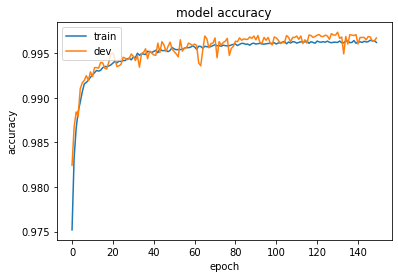
\includegraphics[width=\linewidth]{img/learn1.png}
  \end{subfigure}
  \hfill %%
  \begin{subfigure}[b]{0.6\columnwidth}
    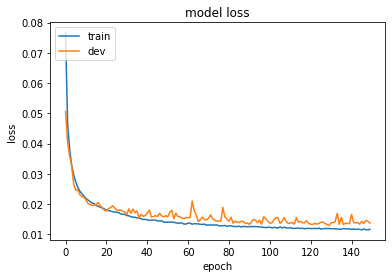
\includegraphics[width=\linewidth]{img/learn2.png}

  \end{subfigure}

      \caption{Learning Curve models of the best model trained on the full data set}
\end{figure}

\begin{table}[h]
\center
\begin{tabular}{|l|l|l||l|l|}
\hline
\multicolumn{3}{|c||}{\textbf{Model}}                                   & \multicolumn{2}{c|}{\textbf{Evaluation}} \\ \hline
\textit{Inputs} & \textit{Selection Algorithm} & \textit{Hidden Units} & \textit{DR}    & \textit{FAR}    \\ \hline
122             & None                         & 80                    &   71.4\%                  &    0.3\%                \\ \hline
122             & None                         & 80, 30                &   68.1\%                 &     0.3\%               \\ \hline
122             & None                         & 30                    &  71.92\%                   &  8.2\%                  \\ \hline
122             & None                         & 50, 10                &   72.61\%                   &   7.6\%                   \\ \hline
122             & None                         & 20                &    67.71\%                 &       7.9\%             \\ \hline
122             & None                         & 10                &    66.89\%                 &     7.7\%               \\ \hline
\end{tabular}
\caption{Comparison between models trained on the full data set}
\label{tab:allfeat}
\end{table}


%-------
\subsection{ExtraTree selected features}

Four different models where tested using ExtraTree Classifier as feature selection algorithm: 2 with the top 80 features and 2 with the top 15 features in the importance ranking. Table~\ref{tab:treefeat} reports the evaluation of each model.


\begin{table}[h]
\center
\begin{tabular}{|l|l|l||l|l|}
\hline
\multicolumn{3}{|c||}{\textbf{Model}}                                   & \multicolumn{2}{c|}{\textbf{Evaluation}} \\ \hline
\textit{Inputs} & \textit{Selection Algorithm} & \textit{Hidden Units} & \textit{DR}    & \textit{FAR}    \\ \hline
80             & ExtraTree                         & 10                    &   61.1\%                  &   7.8\%                 \\ \hline
80             & ExtraTree                         & 30, 10               &   69.29\%                  &    7.6\%                \\ \hline
40             & ExtraTree                         & 10                    &   59.7\%                  &   3\%                 \\ \hline
40             & ExtraTree                         & 30, 10               &   59.5\%                  &     3\%               \\ \hline
15             & ExtraTree                         & 8                &       67.2\%              &   6.86\%                 \\ \hline
15             & ExtraTree                         & 4                &       64.6\%              &   7.3\%                 \\ \hline
\end{tabular}
\caption{Comparison between models trained on ExtraTree selecte features}
\label{tab:treefeat}
\end{table}

%%%%

\begin{figure}[h]
\center
  \begin{subfigure}[b]{0.6\columnwidth}
    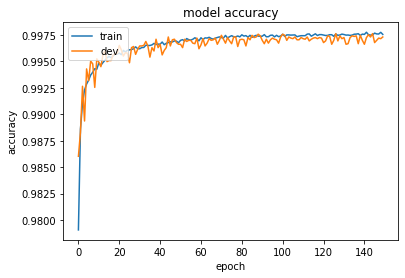
\includegraphics[width=\linewidth]{img/learn3.png}
  \end{subfigure}
  \hfill %%
  \begin{subfigure}[b]{0.6\columnwidth}
 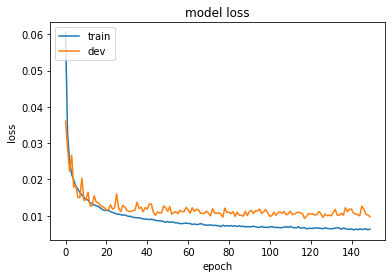
\includegraphics[width=\linewidth]{img/learn4.png}
  \end{subfigure}
\caption{Learning Curve models of the best model trained on Extra Tree selected features}
\end{figure}

%-------
\subsection{Univariate selected features}

Four different models where tested using Univariate Selection as feature selection algorithm: 2 with the top 80 features and 2 with the top 15 features in the importance ranking. Table~\ref{tab:univfeat} reports the evaluation of each model.

\begin{table}[h]
\center
\begin{tabular}{|l|l|l||l|l|}
\hline
\multicolumn{3}{|c||}{\textbf{Model}}                                   & \multicolumn{2}{c|}{\textbf{Evaluation}} \\ \hline
\textit{Inputs} & \textit{Selection Algorithm} & \textit{Hidden Units} & \textit{DR}    & \textit{FAR}    \\ \hline
80             & Univariate                         & 10                    &   66.56\%                  &   7.4\%                 \\ \hline
80             & Univariate                         & 30, 10               &     70\%                &   7.4\%                 \\ \hline
40             & Univariate                         & 10                    &    69\%                 &   7.8\%                 \\ \hline
40             & Univariate                         & 30, 10               &   73.7\%                  &    3.4\%                \\ \hline
15             & Univariate                         & 8                &    57\%                 &      7.4\%              \\ \hline
15             & Univariate                         & 4                &    63.7\%                 &          3.1\%          \\ \hline
\end{tabular}
\caption{Comparison between models trained on Univariate selected features}
\label{tab:univfeat}
\end{table}

%%%%

\begin{figure}[h]
\center
  \begin{subfigure}[b]{0.6\columnwidth}
    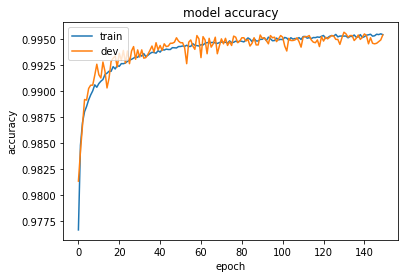
\includegraphics[width=\linewidth]{img/learn5.png}
  \end{subfigure}
  \hfill %%
  \begin{subfigure}[b]{0.6\columnwidth}
 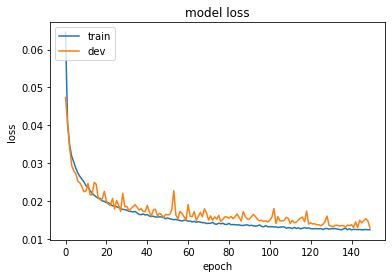
\includegraphics[width=\linewidth]{img/learn6.png}
  \end{subfigure}
\caption{Learning Curve models of the best model trained on Univariate selected features}
\end{figure}


%-------
\subsection{Re-shuffled Train Set}
\label{subsec:porcata}

Given that the results of the preceding models are far from being enough to deploy an IDS in a real network, another approach has been tried. The train and test set have been merged together, split again in train and test set and re-normalized using a normalization based on the train set alone. This approach gave much better results, meaning that probably the test set has many outliers that have to be taken into account when designing the ANN. Figure~\ref{tab:porcata} displays the results of the same models but with the shuffled dataset.

\begin{figure}[h]
\center
  \begin{subfigure}[b]{0.6\columnwidth}
    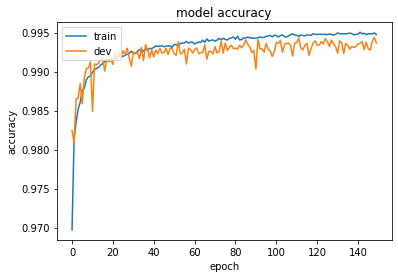
\includegraphics[width=\linewidth]{img/learn7.png}
  \end{subfigure}
  \hfill %%
  \begin{subfigure}[b]{0.6\columnwidth}
 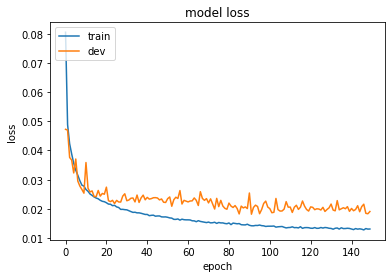
\includegraphics[width=\linewidth]{img/learn8.png}
  \end{subfigure}
\caption{Learning Curve models of the best model trained on the shuffled data set}
\end{figure}

\begin{table}[h]
\center
\begin{tabular}{|l|l|l||l|l|}
\hline
\multicolumn{3}{|c||}{\textbf{Model}}                                   & \multicolumn{2}{c|}{\textbf{Evaluation}} \\ \hline
\textit{Inputs} & \textit{Selection Algorithm} & \textit{Hidden Units} & \textit{DR}    & \textit{FAR}    \\ \hline
122             & None                         & 10                    &   99.18\%                  &   1.2\%                 \\ \hline
122             & None                         & 50, 10               &     99\%                &  0.6\%                 \\ \hline
122             & None                         & 20                    &    98.15\%                 &   0.3\%                 \\ \hline
122             & None                         & 30                    &    99.3\%                 &   0.8\%                 \\ \hline
122             & None                         & 80, 30               &   99.3\%                  &    0.5\%                \\ \hline  \hline
80             & Univariate                         & 10                    &   98.6\%                  &   1.8\%                 \\ \hline
80             & Univariate                         & 30, 10               &     99\%                &   1.1\%                 \\ \hline
40             & Univariate                         & 10                    &    98.18\%                 &   1.8\%                 \\ \hline
40             & Univariate                         & 30, 10               &   98.7\%                  &    1.3\%                \\ \hline
15             & Univariate                         & 8                &    90.9\%                 &      3.2\%              \\ \hline
15             & Univariate                         & 4                &    91.6\%                 &          3.7\%          \\ \hline
\end{tabular}
\caption{DR and FAR with new train/test set splitting}
\label{tab:porcata}
\end{table}

%-------
\section{Deployment in a Network}
\label{chapter:deployment}
This Section describes which steps should be made in order to deploy one or more of the produced models in a real network environment.

\subsection{Sensors}

In order to deploy an IDS in a real network, the first components we need are sensors that are able to record traffic and produce the tuples that will be then fed into the aforementioned model.

Sensor placement is a key factor in an IDS to be able to protect the network from invasion. For this task, the network architecture should be studied in detail, to observe all possible points of entrance.
Depending on how large and complex is our network, we can choose to deploy the whole system in a single device, as suggested by \cite{dpl}, or implement multiple sensors as done in \cite{dpl2}.

In both cases, the most sensitive points where to place the sensors are typically before and after each router or DMZ of the network. Figure~\ref{fig:dpl} describes this situation.

\begin{figure}[h]
    \centering
    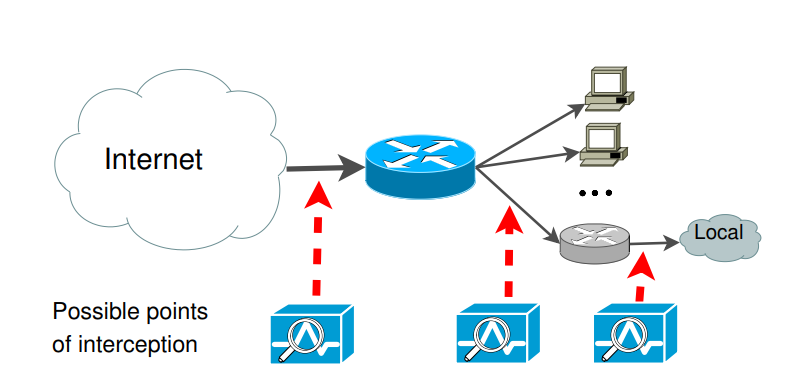
\includegraphics[width=\linewidth]{img/dpl.png}
    \caption{Possible points of interception for a NIDS}
    \label{fig:dpl}
\end{figure}

Generally, IDS sensors have two network interfaces — one for monitoring traffic and one for management. The traffic-monitoring interface is unbound from any protocol, which means that the interface has no IP address and other entities can't communicate with it. This guarantees that no attack surface is exposed on the network by the sensor itself.

\subsection{Model Choice}

After deploying the sensors, we have to choose which model to deploy. The model choice can depend on evaluation metrics like Detection Rate or False Alam Rate, but should also take into account the model complexity. A higher model complexity can in fact imply a higher cost for data acquisition and higher delays for the system's response. This kind of analysis shall be done taking into consideration also the time of response of each model, which is out of the scope of this work.

For reducing the complexity we can employ one of the Feature Selection methods described in Section~\ref{chapter:feature-selection}.

\subsection{Model Deployment}

Once the IDS is deployed in the network, we want it to work with streams of incoming data in a fully automated way. This implies several steps, which are described in Figure~\ref{fig:dplsteps}.

\begin{figure}[h]
    \center
    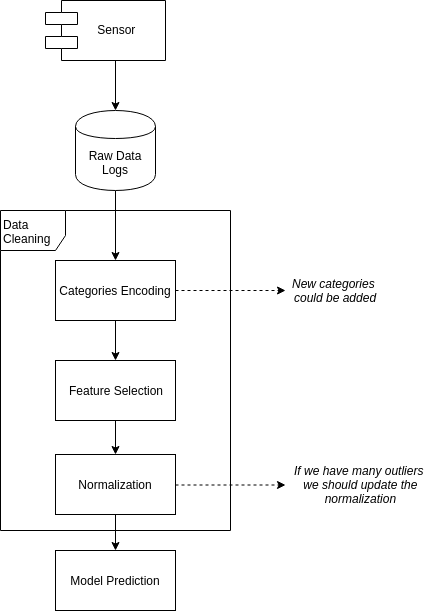
\includegraphics[width=\linewidth]{img/ids-dpl.png}
    \caption{Steps of the IDS once deployed}
    \label{fig:dplsteps}
\end{figure}

There are many possible solutions, to achieve this automation, which range from fully personalized solutions to fully COTS products. One simple possibility, since the models of this work have been trained using TensorFlow, is to use TensorFlow \textit{Extend} \cite{tfx}, a collection of tools used for deploying ANN models in the wild. Figure~\ref{fig:tfx} describes the components of the TFX framework, which range from data cleaning to Keras model validation.

\begin{figure}[h]
    \centering
    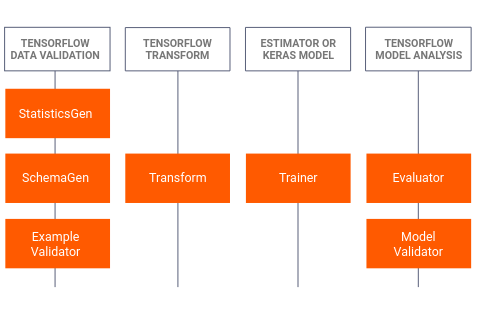
\includegraphics[width=\linewidth]{img/tfx.png}
    \caption{Image taken from \url{https://www.tensorflow.org/tfx/guide}}
    \label{fig:tfx}
\end{figure}

On-Line deployment can be achieved by using \textit{TensorFlow Serving} \cite{tfserve}, which is a framework built to enable fast TensorFlow models' deployment over REST APIs. TF Serving also has the possibility to deploy an ML model in a Docker image and use Kubernetes to manage a cluster of these images running together. This offers a good solution in terms of scalability of the IDS, which is able to easily keep up with a possible growth of the network that it's protecting.

\subsection{Model Adaptation}

Once it is online, the model should be then trained and updated with real data coming from the network. This is a time-consuming task, which requires the network to be in a temporary 'safe' state in which the model can learn which is the normal behaviour of the system. After the training time, the IDS is ready to be used in the network environment.

To extend the training time, a human supervisor can be assigned to checking the entries that are signaled as \textit{anomalous} and relabelling them if necessary. The same model can also be periodically retrained with a larger dataset or with only the latest entries.

%-------
\section{Future Work}
\label{chapter:future}

This work represents only a preliminary analysis of how a NIDS can be modelled and deployed using ANN and TensorFlow.

Many improvements can be made to the models in order to get better performances, such as implementing early stopping instead of a fixed amount of epochs and adapt the keras model to work with TPUs (Tensor Processing Units) which can significantly improve the training time needed.

Also, an in-depth analysis of a target network should be performed in order to deploy the IDS in a real network. Problems as the efficiency, delay and the samples collection in the new network environment are specific of each network, and have to be taken into account if we want to carry out the IDS deployment.


\bibliographystyle{unsrt}
\bibliography{references}

\end{document}
